
\chapter{FUNDAMENTAÇÃO TEÓRICA} \label{cap:funda}

Nessa seção é descrito o estado da arte do tema escolhido. Primeiramente é dado uma breve introdução sobre processamento de imagem, dando maior ênfase no processo de análise de imagem, seguindo teoria de \citeonline{GONZALEZ1992}. Este capítulo também será utilizado para descrever o funcionamento de um sistema OCR.

\section{Processamento Digital de Imagens}


Segundo \citeonline{Huang1996} visão computacional possui um propósito duplo. Partindo de um ponto de vista biológico, visão computacional é o estudo dos modelos computacionais do sistema visual humano. Já partindo de um ponto de vista de engenharia, visão computacional tem o objetivo de criar sistemas autônomos capazes de executar tarefas que o sistema visual humano executa, e em alguns casos até supera.


Para \citeonline{PEDRINI2008}, a visão computacional pode ser dividida em dois níveis de abstração: processamento de imagens (baixo nível) e análise de imagens (alto nível). O processamento digital de imagens pode ser determinado como um conjunto de técnicas para capturar, representar e transformar imagens utilizando um computador. A aplicação dessas técnicas permite extrair e identificar informações das imagens e melhorar a qualidade visual de aspectos estruturais, simplificando a percepção humana e a interpretação automática por meio de máquinas \cite{PEDRINI2008}. Essa abordagem, de baixo nível, utiliza técnicas como o aumento de contraste, a redução de ruído, a extração de bordas e a compressão de imagens.

De acordo com \citeonline{GONZALEZ2002}, a área de PDI vem evoluindo constantemente no decorrer dos anos, com uma ampliação significativa dos estudos envolvendo morfologia matemática, redes neurais, processamento de imagens coloridas, compressão de imagens, reconhecimento de imagens e sistemas de análise de imagens baseados em conhecimento.


O objeto de operação do Processamento Digital de Imagens são as imagens digitais. Uma imagem na forma digital é representada por meio de matrizes, as quais mapeiam as cores reais da imagem, do mundo físico para o digital \cite{Almeida2018}.





Os sistemas de PDI consistem em um conjunto de técnicas que possibilitam a captura de imagens por meio de equipamentos variados, como tomógrafos médicos, câmeras fotográficas, satélites e outros, tal como a representação e transformação destas imagens. O propósito é fazer a extração e identificação das informações que fazem parte das imagens, de forma automática por meio de máquinas \cite{PEDRINI2008}.

% EM TODAS AS SEÇÕES VOCÊ DEVERÁ TRAZER ARTIGOS QUE APLICARAM OS TEMAS DAS SEÇÕES E COMENTAR SOBRE O OBJETIVO E RESULTADO OBTIDOS NESTES TRABALHOS.
%fabiano: tentei encaixar autores relevantes em muitas afirmações. está faltando algum?

% EVERTON: Veja a seção 2.1. Você apenas referenciou o tema. É importante que você traga artigos onde o tema da seção foi utilizado e aplicado, trazendo a colaboração e resultado do artigo. Por exemplo> fulano de tal utilizou tal coisa e em seus estudos foi possível ..... É preciso ter referencial assim para todas as suas fundamentações.


\subsection{Representação de Imagens Digitais}
% EVERTON: Você fala sempre deste Gonçalves, não tem outras fontes? Para não ficar direcionado? Talvez buscar por quem tenha utilizado trabalho dele também. Quando se refere a elementos de uma função, coloque em itálico: m, n, M, N, f(x,y)....

Segundo \citeonline{Goncalves2016}, uma imagem pode ser representada no plano cartesiano por uma função f(x,y), onde x e y são coordenadas espaciais. A função f(x,y) possui, comumente, um valor em níveis de cinza, ou cor, em qualquer ponto da imagem. O ponto de origem representado pela coordenada (0,0) fica situado no canto superior esquerdo da imagem.




A Figura \ref{img1} ilustra como seria um imagem digital em forma de notação matricial. Os elementos dessa matriz são chamados de elementos pictóricos, elementos de imagens, pels e pixel. O \textit{Pixel} (contração de Picture element) é o termo mais utilizado \cite{GONZALEZ2006}. O índice m representa a linha na qual o pixel se encontra, enquanto que o índice n aponta a coluna na qual está localizado o pixel. Em uma imagem M linhas e N colunas, m terá seu valor variando de 0 até M-1 e n terá seu valor variando de 0 até N-1 \cite{Almeida2018}. 

 \begin{figure}[h!]
	\centering
	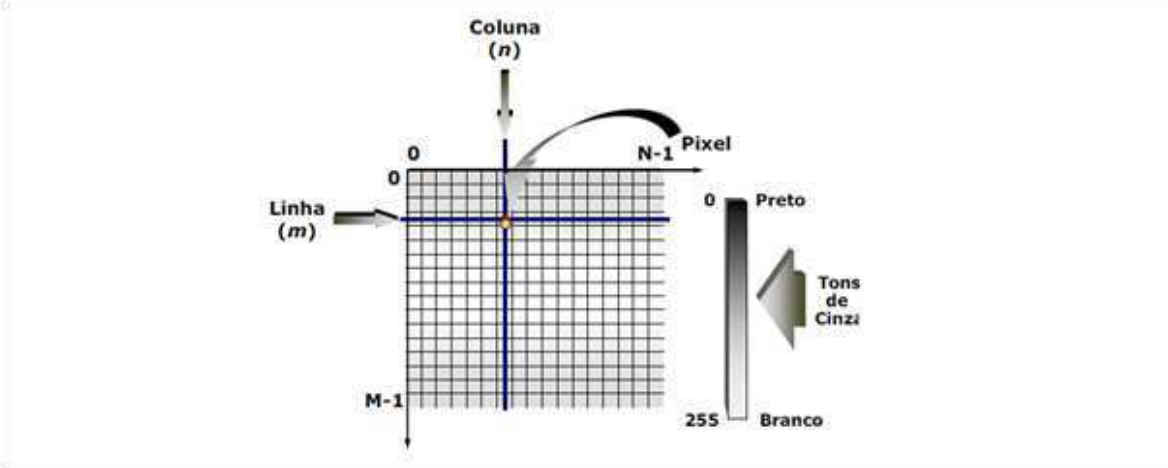
\includegraphics[width=0.85\textwidth]{Imagens/imagem1} 
	\caption[Representação da imagem em uma matriz bidimensional.]{Representação da imagem em uma matriz bidimensional.}
\fonte{\citeonline{Goncalves2016}}
	\label{img1}
\end{figure}

Segundo \citeonline{PEDRINI2008} uma imagem digital pode ser representada por meio de uma matriz bidimensional, na qual cada pixel da imagem corresponde a um elemento da matriz. Na Figura~\ref{fig:imagem6} é possível ver um exemplo de representação matricial de uma imagem, sendo que uma pequena região destacada é formada por números inteiros que representam o nível de cinza dos pixels da imagem. Existem várias vantagens ao utilizar matrizes para representação de imagens, pois são estruturas simples para armazenar, manipular e visualizar dados \cite{PEDRINI2008}. 

 \begin{figure}[h!]
	\centering
	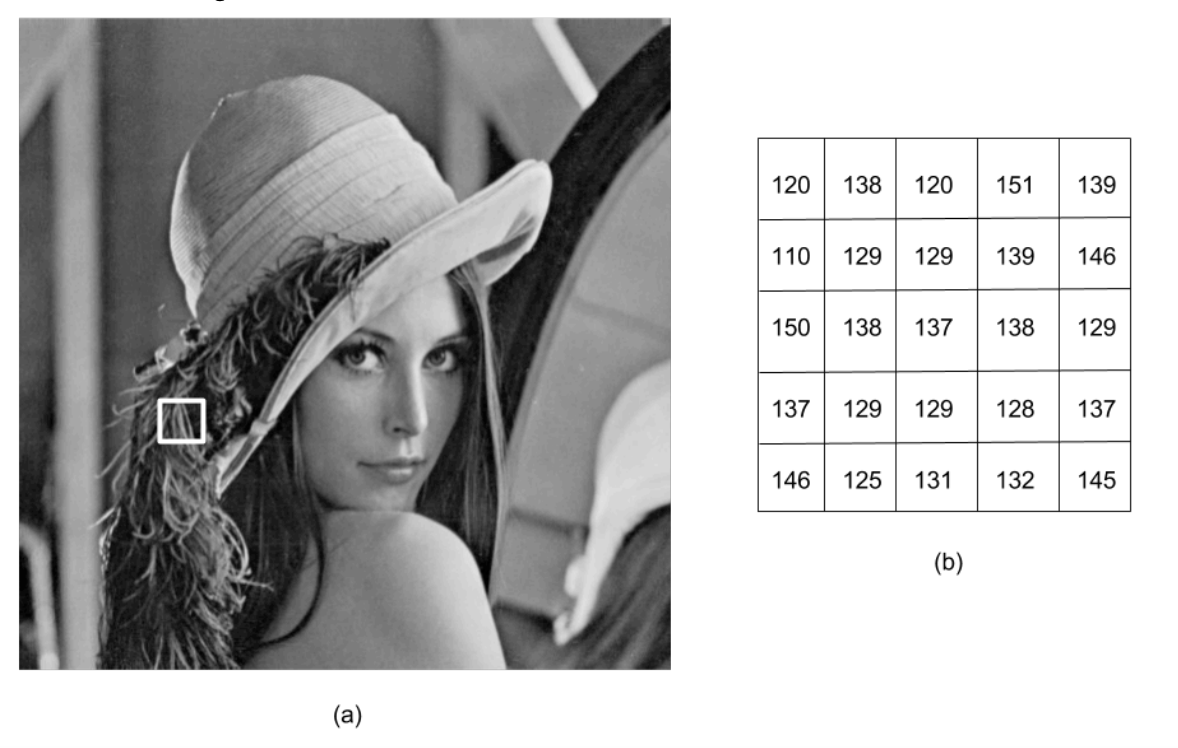
\includegraphics[width=0.7\textwidth]{Imagens/imagem6} 
	\caption[Representação matricial;]{Representação matricial; (a) imagem; (b) níveis de cinza correspondentes a região
destacada da imagem.}
\fonte{\citeonline{PEDRINI2008}}
	\label{fig:imagem6}
\end{figure}


Em uma imagem digital existem vários relacionamentos importantes entre os pixels. Conforme descrito em \citeonline{GONZALEZ2002}, 
um pixel p de coordenadas (x,y) possui uma vizinhança horizontal e vertical determinadas por (x-1, y), (x+1, y) e (x, y-1), (x, y+1) denominada vizinhança-4, e também uma vizinhança diagonal composta pelas coordenadas (x-1, y-1), (x-1, y+1), (x+1, y-1) e (x+1, y+1), convencionado com o nome de vizinhança-8 a união destas vizinhanças.

Quando o pixel p estiver localizado na borda da imagem, alguns dos pixels vizinhos não estarão presentes na imagem. Isto pode ser mais bem entendido analisando-se a figura~\ref{fig:imagem3} que demonstra visualmente o conceito de vizinhança de um pixel.

 \begin{figure}[h]
	\centering
	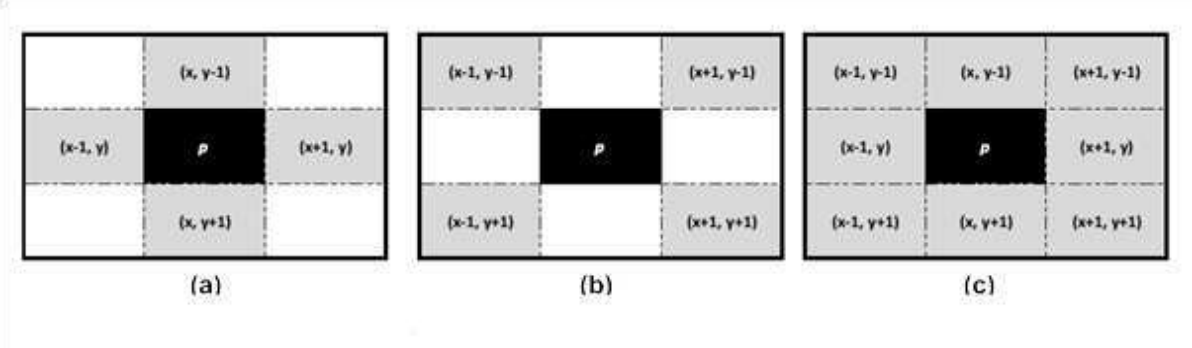
\includegraphics[width=1.0\textwidth]{Imagens/imagem3} % <- formatos PNG, JPG e PDF
	\caption[Texto que vai aparecer na lista de fig.]{Tipos de vizinhança. (a) Vizinhança-4; (b) Vizinhança diagonal; (c) Vizinhança-8.  (a) Imagem; (b) Histograma.}
\fonte{\citeonline{Goncalves2016}}%citaç\~ao do livro onde pegou a figura	
	\label{fig:imagem3}
\end{figure}

A conectividade entre pixels é um conceito importante no processamento de imagens, em especial para o reconhecimento de bordas de objetos presentes em uma imagem. Para identificar se dois pixels são conexos, é preciso averiguar se são vizinhos e se seus níveis de cinza são similares \citeonline{Goncalves2016}. É fundamental analisar a possibilidade de haver conexidade por meio da utilização da vizinhança-4 ou utilizando a vizinhança-8.




\section{Ciclo de Gonzalez}
%EVERTON: Veja a data da sua referência quando fala das últimas décadas. Tem um comentário do PEDRO no meio do texto
Os dispositivos desempenham um papel essencial em um sistema de processamento de imagem, podendo ser utilizados para aquisição, armazenamento, processamento, transmissão e exibição de imagens. Com o crescente avanço tecnológico e a demanda de certas áreas de aplicação, estes dispositivos têm evoluído de forma significativa nas últimas décadas \cite{PEDRINI2008}.
%(PEDRO: atualizar imagem conforme livro de 2018)
% slide 11 de link abaixo, tem a 3a edição, você pode buscar no google images ou books caso queira a 4a edição:
% https://www.slideshare.net/asodariyabhavesh/chapter-1-and-2-gonzalez-and-woods

Segundo \citeonline{GONZALEZ1992}, as técnicas em análise de imagem podem ser divididas em três áreas básicas: (1) aquisição e processamento de baixo nível, com funções que podem ser vistas como reações automáticas, ou seja, reações que não requerem comportamento inteligente; (2) processamento de nível intermediário, com processos de extração e caracterização de componentes em uma imagem; e (3) processamento de alto nível, que envolve os processos de reconhecimento e interpretação. A figura~\ref{fig:imagem5} mostra os processos de cada uma dessas áreas.

% ToDo: aqui tem algo que pode ser útil para rodar python no IOS:
% https://beeware.org/project/using/ios-app/

 \begin{figure}[h]
	\centering
	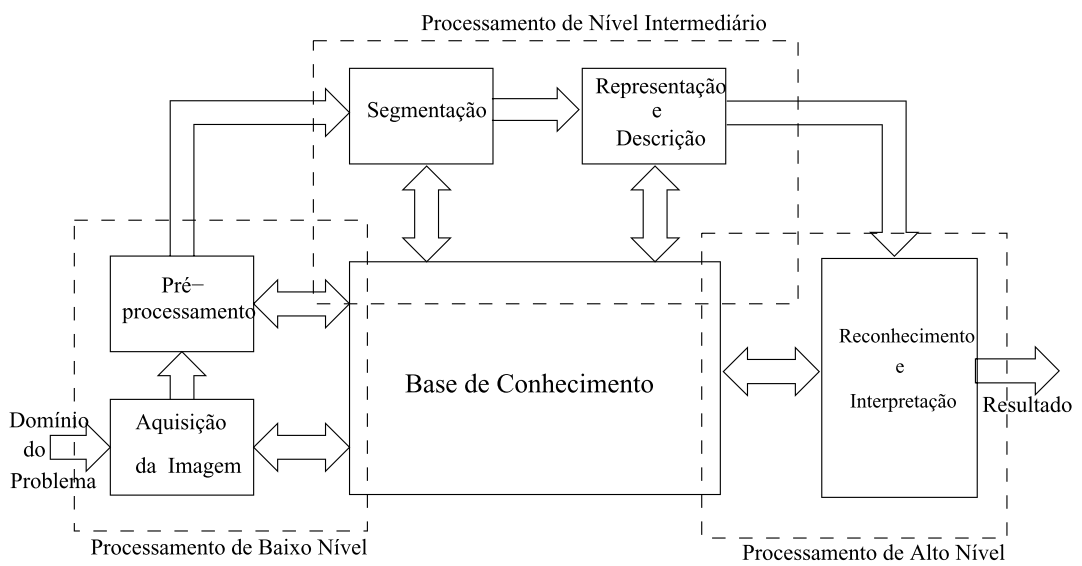
\includegraphics[width=1.0\textwidth]{Imagens/imagem5} % <- formatos PNG, JPG e PDF
	\caption[Elementos do processo de análise de imagem.]{Elementos do proceso de análise da imagem. }
\fonte{\citeonline{GONZALEZ1992}}%citaç\~ao do livro onde pegou a figura	
	\label{fig:imagem5}
\end{figure}



% EVERTON: cuidado que daqui pra frente está parecendo metodologia, como se faz. Aqui é referencial teórico
O primeiro passo do processo de reconhecimento é a aquisição da imagem. Segundo \citeonline{GONZALEZ1992}, o primeiro passo do processo requer apenas um sensor de imagens e a capacidade para digitalizar o sinal produzido pelo
sensor. O sensor converte a informação óptica em um sinal elétrico e o digitalizador transforma a imagem analógica em imagem digital. A imagem resultante pode apresentar diversas imperfeições, tais como: presença de pixels ruidosos, contraste e/ou brilho inadequado, etc (MARQUES;VIEIRA, 1999).

Após a aquisição e digitalização da imagem, o próximo passo é o pré-processamento. A função chave do pré-processamento é melhorar a imagem, com o objetivo de aumentar as chances de sucesso dos processos seguintes \cite{GONZALEZ1992}. Nesta etapa, são utilizadas técnicas para aumento de contraste, remoção de ruídos, realce e normalização, com o objetivo de converter os padrões para uma forma que possibilite uma simplificação do processo de reconhecimento \cite{Rodrigues2002}.

O próximo estágio é o processo chamado de segmentação. A segmentação de imagens, demonstrado na figura~\ref{fig:segmentacao} consiste em dividir uma imagem em suas unidades significativas, para uma melhor caracterização das regiões de interesse (\sigla{ROI}{Região de Interesse}). As operações de segmentação procuram isolar regiões de pontos da imagem pertencentes a objetos, para posterior extração de atributos \cite{Lourdes2010}.
 \begin{figure}[h]
	\centering
	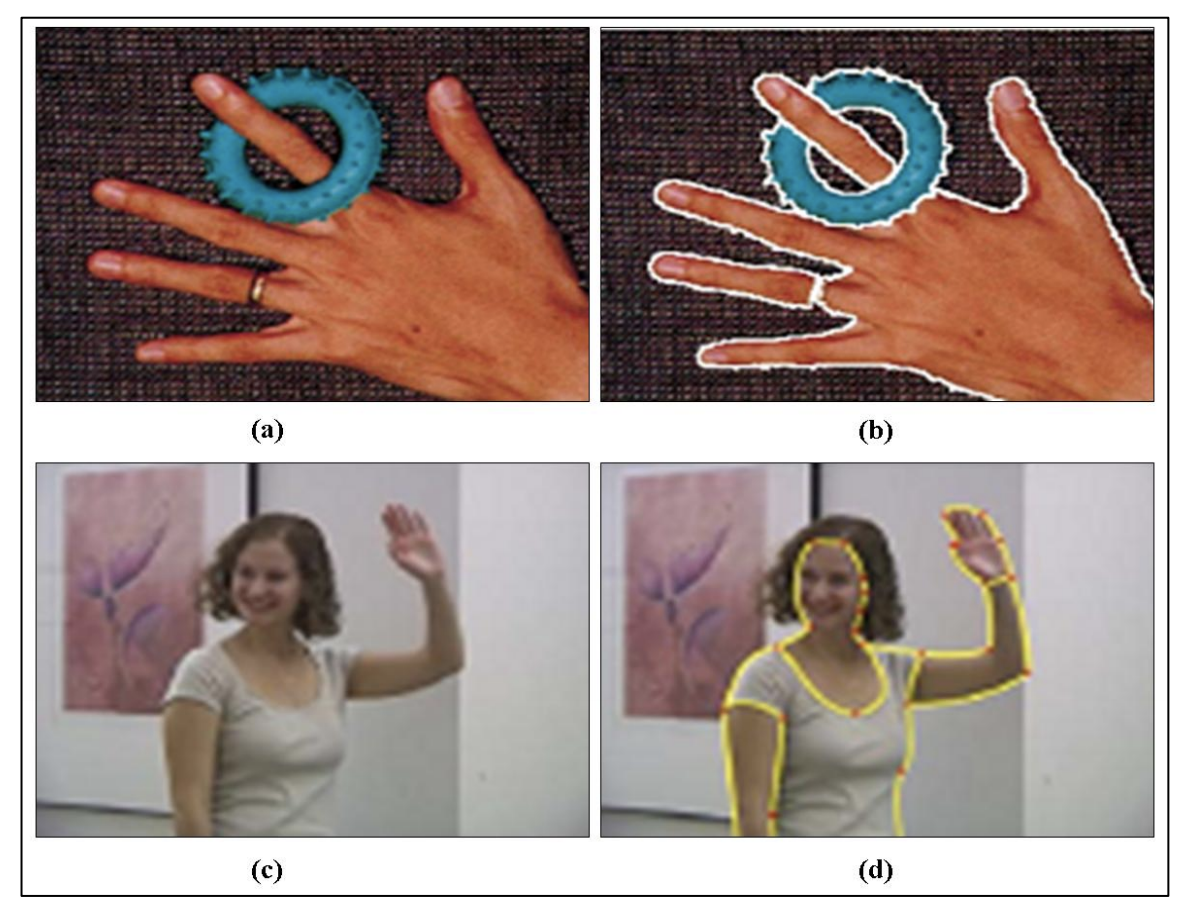
\includegraphics[width=1.0\textwidth]{Imagens/segmentacao} % <- formatos PNG, JPG e PDF
	\caption[Segmentação de Imagens: (a) imagem original, (b) imagem após segmentação; (c) imagem original; (d)imagem após segmentação.]{Segmentação de Imagens: (a) imagem original, (b) imagem após segmentação; (c) imagem original; (d)imagem após segmentação.}
\fonte{\citeonline{SZELISKU2010}}%citaç\~ao do livro onde pegou a figura	
	\label{fig:segmentacao}
\end{figure}
De um modo geral, as técnicas de segmentação utilizam duas abordagens principais: a similaridade entre os pixels e a descontinuidade entre eles. A binarização de imagens, técnica baseada em similaridade, é a técnica mais utilizada, é uma  simples e eficiente técnica do ponto de vista computacional, sendo portanto comumente utilizada em sistemas de visão computacional \cite{ISRAEL2003}.

Na segmentação com descontinuidade entre os pixels, a segmentação é baseada nas técnicas de limiarização, crescimento por regiões, união e divisão de regiões \cite{Rodrigues2002}.  % VEJA QUE AQUI E EM OUTROS PONTOS VOCÊ TRAZ TERMOS ESPECÍFICOS, QUE PODERIAM SER EXPLICADOS EM SEU TEXTO.

A etapa de segmentação é seguida por uma etapa de representação e descrição, na qual, através de descritores, busca-se obter um conjunto de dados correspondentes àquela imagem.

Normalmente, após a segmentação, dados brutos de pixel são obtidos. Por consequência, pode ser fundamental o processo de converter os dados para uma forma apropriada, possibilitando o processamento digital. 

Dois tipos de representação podem ser utilizados: representação limite ou representação regional. Quando o foco está com características de localização nas extremidades, como por exemplo cantos e bordas da imagem, é apropriada a representação limite. Representação regional é apropriada quando o foco está localizado no centro da imagem e é possível encontrar uma vizinhança-8. Escolher a representação é apenas uma parcela da solução para a conversão de dados brutos em uma forma adequada para o processamento computacional. \cite{Rodrigues2002}
%EVERTON: Estou preocupado com a época das referências. São muito antigas. Nada mudou neste período?

O ultimo estágio no processo de análise da imagem envolve reconhecimento e interpretação. Reconhecimento é o processo que fixa um rótulo a um objeto baseado na informação extraída na etapa anterior. Interpretação envolve a fixação de significado a um grupo de objetos reconhecidos. Para resolver problemas de reconhecimento pode-se partir de três abordagens: estatística, estrutura e neural \cite{GONZALEZ1992}.

Todas as etapas descritas pressupõem a existência de um conhecimento sobre o problema a ser resolvido, armazenado em uma base de conhecimento, cujo tamanho e complexidade podem variar enormemente. Idealmente, esta base de conhecimento deveria não somente guiar o funcionamento de cada etapa, mas também permitir a realimentação entre elas, \cite{marques1999}.


\section{Detecção de Bordas}

Segundo \citeonline{Antonio}, uma borda é definida por uma mudança repentina do nível de cinza, ou seja ocorre uma descontinuidade no tom de cinza. Dessa forma, a descontinuidade pode ser percebida quando o gradiente da imagem tem uma brusca variação. Para \citeonline{PEDRINI2008}, a detecção de bordas é o limite entre duas regiões com propriedades razoavelmente distintas de nível de cinza. \citeonline{SZELISKU2010}, define que uma borda é uma fronteira entre regiões de diferentes cores, intensidades ou texturas. Já \citeonline{marques1999} definem borda como uma descontinuidade na luminosidade de uma imagem.

Para \citeonline{Silva2001}, é possível considerar o pixel como borda calculando o gradiente deste pixel e, caso o gradiente seja maior do que um valor de limiar pré-definido, o pixel é considerado como borda. 

Para \citeonline{GONZALEZ2002}, a ideia associada à maioria das técnicas para a detecção de bordas é o cálculo de um operador local diferencial que seja sensível a mudanças ou descontinuidade nos níveis de cinza. Um operador de derivada pode ser usado para executar essa função, visto que se poderia avaliar a taxa de mudança da função dos níveis de cinza. A taxa de mudança dos níveis de cinza em uma imagem tende a ser maior perto das bordas e menor em áreas constantes, caracterizando as bordas como os pontos máximos da derivada \cite{PEDRINI2008}.

Segundo \citeonline{Franco2013}, diversas abordagens foram propostas ao longo dos anos para a detecção de bordas em imagens digitais, como por exemplo, os operadores de Roberts, Hough, Sobel e Canny. A abordagem utilizada nesse trabalho é a transformada de Hough. Segundo \citeonline{PEDRINI2008}, o método de Hough é altamente eficiente na detecção de bordas em linhas retas.
%EVERTON: A abordagem utilizada nesse trabalho é a transformada de Hough isso deverá estar no MATERIAL E MÉTODOS se for sobre seu trabalho.

Na detecção de linhas retas, \citeonline{SZELISKU2010} diz que parte da complexidade inerente à detecção de linhas retas em imagens vem do fato de que, no mundo real, as linhas são normalmente compostas por componentes desconectados ou mesmo feitas de diversos segmentos colineares, sendo necessário agrupá-los para possibilitar a detecção. Em diversas áreas de PDI surge o problema da determinação da localização e orientação de linhas retas em imagens.
%EVERTON: O texto Em diversas áreas de PDI surge o problema da determinação da localização e orientação de linhas retas em imagens. parece largado. Sem ligação com o que vinha sendo dito.

\citeonline{PEDRINI2008} citam que o problema na detecção de linhas retas consiste essencialmente em achar subconjuntos de pontos que sejam colineares e que o método conhecido como Transformada de Hough é eficiente nesta tarefa. A transformada de Hough vem sendo usada para esta finalidade em imagens binárias, onde seu princípio básico é a conversão de coordenadas de um ponto no plano cartesiano em parâmetros em que descrevem este ponto em termos de inclinação e distância de um ponto de origem.


A transformada de Hough é capaz de detectar grupos de pixeis que pertencem a uma linha reta (mesmo que esteja quebrada e/ou com ruídos). Uma linha reta é geralmente descrita como y = mx + b. As características desta reta são a inclinação m e a intersecção b. Assim, uma reta y = mx + b pode ser representada como um ponto (b, m) no espaço dos parâmetros \cite{HOUGHKIM}. 

Porém, ambos parâmetros são ilimitados, isto é, à medida em que a reta torna-se vertical, as magnitudes de b e m tendem ao infinito. Para um bom desempenho computacional, é melhor parametrizar as retas usando dois outros parâmetros, assim transformando a equação da reta na forma polar $(\theta, \rho)$, dada a Equação~\ref{eq:eqreta},

\begin{equation}
\rho = x*\cos{\theta} + y*\sin{\theta}
\label{eq:eqreta}
\end{equation}

$(\rho)$ é a distancia perpendicular da origem (0,0) à reta e $(\theta)$ é o angulo formado entre a reta perpendicular e o eixo x, o espaço $(\theta, \rho)$ deve ser discretizado de modo a permitir sua implementação conforme figura ~\ref{fig:eqreta}. Como $(\theta)$ é medido em relação ao eixo x, os valores possíveis variam de 0$^{\circ}$ a 180$^{\circ}$ e uma discretização com incremento de 1$^{\circ}$ deixaria 181 ângulos possíveis \cite{PEDRINI2008}.

De acordo com \citeonline{GONZALEZ2002}, as principais vantagens da transformada de Hough é que mesmo segmentos que apresentem regiões obstruídas por outros objetos podem ser detectados, e sua baixa sensibilidade à ruído, já que os pontos de uma imagem corrompidos por esse ruído dificilmente serão mapeados em uma mesma célula de acumulação.

 \begin{figure}[h]
	\centering
	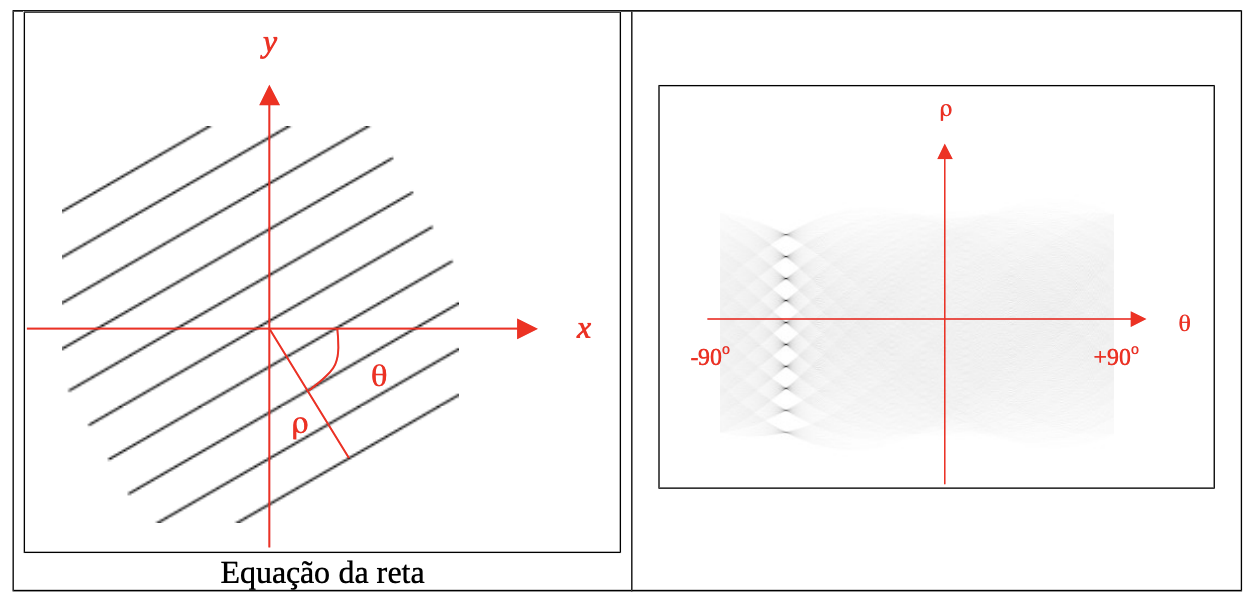
\includegraphics[width=1.0\textwidth]{Imagens/eqreta} 
	\caption[Representação de uma reta através de coordenadas polares.]{Representação de uma reta através de coordenadas polares.}
\fonte{\citeonline{HOUGHKIM}}	
	\label{fig:eqreta}
\end{figure}


\section{Correção de Perspectiva}

Segundo \citeonline{Silveira2006}, a distorção da imagem ocorre devido a diferentes aspectos durante sua captação. A distância entre o plano do objeto e o capturador de imagens promove um erro de perspectiva. Esse tipo de erro pode ser minimizado por meio do posicionamento do segmento de interesse próximo à tela. A correção de erros de perspectiva é desenvolvida por métodos geométricos de relativa simplicidade e vem sendo amplamente utilizada em imagens de raio x. Indo na direção de estruturas de menor escala, a correção de perspectiva é aplicada em processos de digitalização de documentos, onde a correção de distorções na imagem, acarreta em uma maior capacidade de reconhecimento de caracteres em um texto digitalizado \cite{Pereira}. 

A imagem 7 mostra dois exemplos de imagens distorcidas, capturadas por uma câmera digital de baixa resolução e suas respectivas correções. Há uma grande variedade de programas e aplicativos capazes de corrigir as distorções de perspectiva em imagens. Ainda que os programas consigam corrigir as distorções por perspectiva de maneira satisfatória, a correção não se dá em tempo real, além de requerer uma interface gráfica com o usuário para que a correção seja feita.
 \begin{figure}[!h]
	\centering
	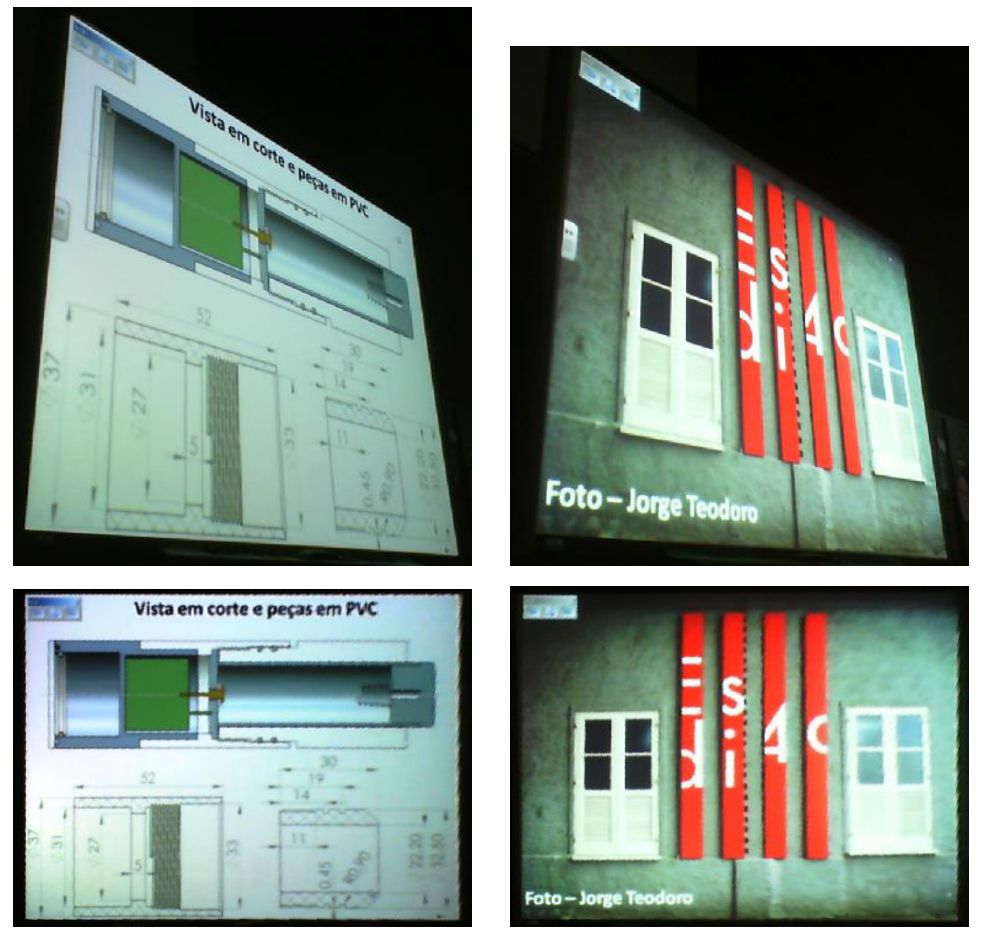
\includegraphics[width=1.0\textwidth]{Imagens/imagensdistorcidas} 
	\caption[Imagens distorcidas e corrigidas.]{Imagens distorcidas (acima) e corrigidas (abaixo).}
\fonte{\citeonline{Pereira}}	
	\label{fig:tux_laplace}
\end{figure}

\citeonline{ZHANG2007} Abordam uma proposta de automatização de correção de imagens fotográficas de quadros brancos.A detecção dos limites formados pelo quadrilátero de uma projeção ou de um quadro branco é o principal obstáculo para a realização de um sistema automatizado de correção de distorções de perspectiva. Os procedimentos descritos por \citeonline{ZHANG2007} são mostrados na figura~\ref{fig:metodologiacorrecao}, onde a transformada de Hough é usada para a detecção dos limites do quadro ou projeção.

 \begin{figure}[h]
	\centering
	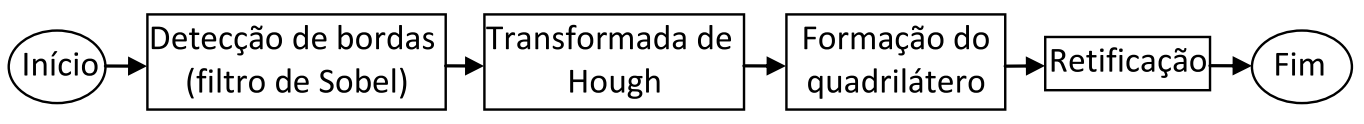
\includegraphics[width=1.0\textwidth]{Imagens/metodologiacorrecao} 
	\caption[Metodologia de detecção.]{Metodologia de detecção.}
\fonte{\citeonline{Pereira}}	
	\label{fig:metodologiacorrecao}
\end{figure}

A detecção do contorno de uma imagem está sujeita às condições de luminosidade do ambiente que podem impor limites na detecção automática do contorno, um algoritmo de detecção de contorno deve apresentar boa imunidade a variações de iluminação do ambiente. \cite{Pereira}.

%//TODO estudos nao finalizados. tópico importante: four_point_transform

\section{RECONHECIMENTO ÓPTICO DE CARACTERES (OCR)}
Reconhecimento óptico de caracteres (OCR) é uma tecnologia que utiliza mecanismos de aquisição, tais como câmeras fotográficas, filmadoras e afins para capturar imagens e posteriormente realizar processamentos nestas para reconhecer caracteres alfanuméricos presentes. Essa tecnologia tenta se aproximar do sistema visual humano, porém ainda não é capaz de competir com a capacidade de leitura deste \cite{Mithe2013}.

 Existem diversas técnicas de identificação automática, na qual cada uma satisfaz às necessidades de sua área de aplicação. Reconhecimento de voz, tarja magnética, código de barra, impressão digital e OCR são exemplos de aplicações que utilizam tecnologias de identificação automática. Segundo \citeonline{Bhatia2014}, os sistemas de OCR são aqueles capazes de transformar uma grande quantidade de documentos, tanto impresso como manuscrito, em texto de máquina codificado. O reconhecimento de caracteres pode ser desempenhado off-line, onde ocorre após a escrita ou impressão do documento estiver finalizada, porém o reconhecimento também pode ser on-line onde o computador reconhece os caracteres na maneira que eles vão sendo desenhados \cite{Eikvil1993}. A figura~\ref{fig:areaocr} mostra as possíveis etapas para o reconhecimento de caracteres.

%EVERTON: Troque no parágrafo anterior a palavra desempenhado. Seria realizado?
 \begin{figure}[h]
	\centering
	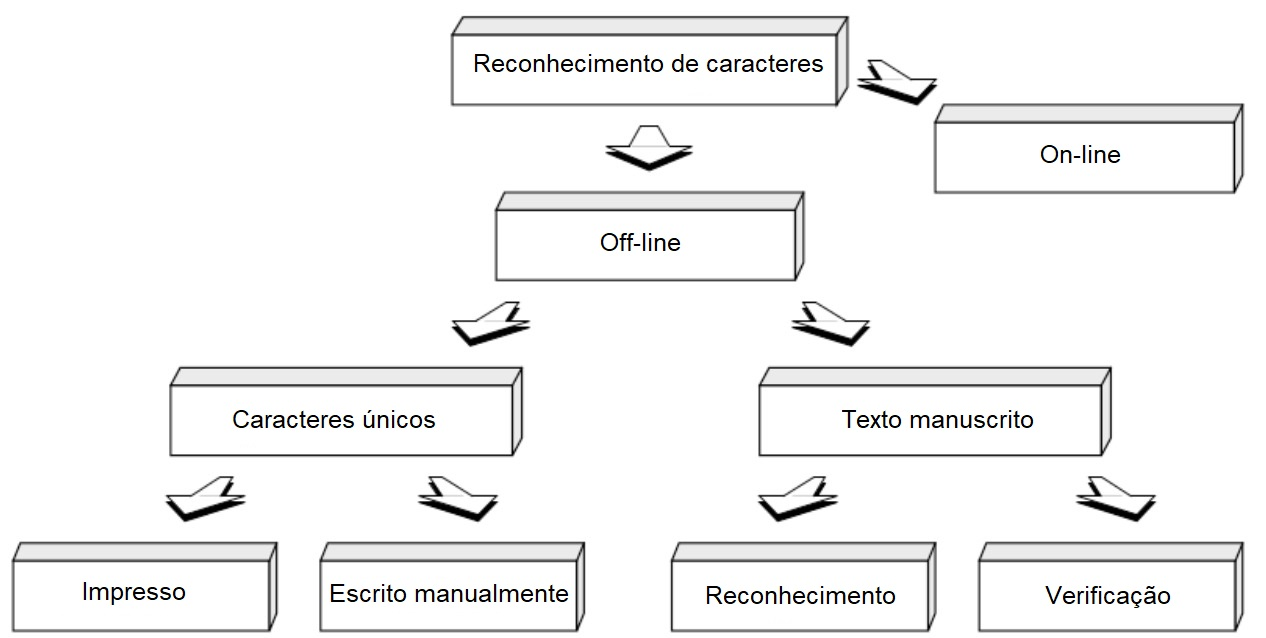
\includegraphics[width=1.0\textwidth]{Imagens/areasocr} 
	\caption[Diferentes áreas de reconhecimento de caracteres.]{Diferentes áreas de reconhecimento de caracteres.}
\fonte{\citeonline{Eikvil1993}}	
	\label{fig:areaocr}
\end{figure}

Para \citeonline{Eikvil1993}, o princípio fundamental para o reconhecimento
automático de caracteres é ensinar a máquina padrões que podem ocorrer e como eles se assemelham. No caso do OCR, os padrões são letras, números e alguns símbolos especiais como vírgulas, pontos de interrogação, entre outros. O ensino da máquina é feito por meio de amostragem de exemplos de textos com as devidas correspondências.
Com base nesses exemplos a máquina constrói um protótipo ou uma
descrição de cada classe de caracteres. Então, durante o reconhecimento, os caracteres desconhecidos são comparados com os anteriormente aprendidos, e então se atribuiu a melhor correspondência \cite{Eikvil1993}.
% EVERTON: Cuidado no uso de "através". Muitas vezes é "por meio". Veja no final do parágrafo anterior "atribuiu". Está certo? Não é"atribui"?

\subsection{Componentes de um sistema OCR}
Um sistema típico de OCR consiste em diversos componentes, podendo variar de
acordo com a aplicação e a metodologia utilizada. 
Para \citeonline{Eikvil1993}, um sistema de OCR é composto pelos seguintes componentes: escaneamento ótico, localização e segmentação, pré-processamento, extração de características, classificação e pós-processamento. Já para \citeonline{Goswami2013}, um sistema típico de OCR consiste em 6 componentes, conforme demonstrado na figura~\ref{fig:etapasocr}, envolvendo as etapas do reconhecimento de caracteres.



 \begin{figure}[h]
	\centering
	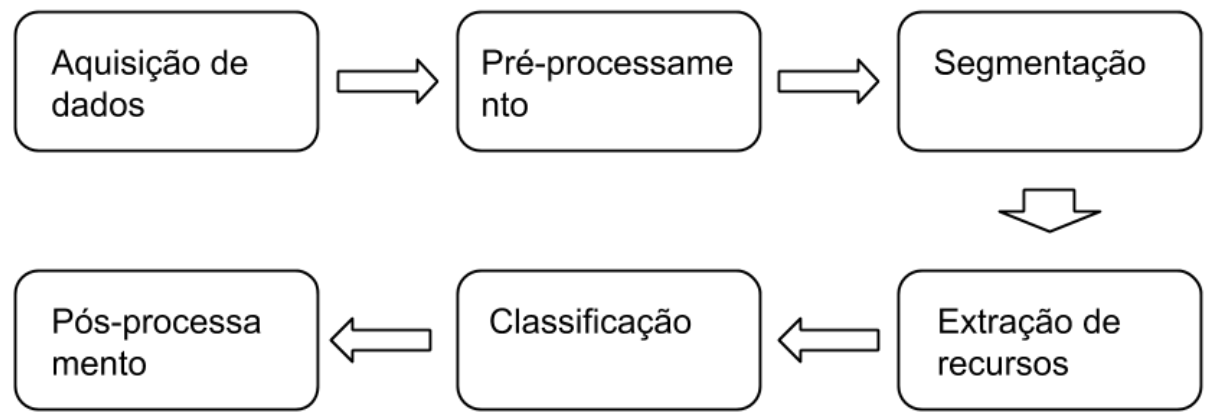
\includegraphics[width=1.0\textwidth]{Imagens/etapasocr} 
	\caption[Sequência de etapas em um sistema OCR.]{Sequência de etapas em um sistema OCR.}
\fonte{\citeonline{Goswami2013}}	
	\label{fig:etapasocr}
\end{figure}

Segundo \citeonline{Goswami2013}, a primeira etapa é a aquisição de dados, que pode ser feita por meio de um escaneamento óptico, capaz de realizar a transformação de um documento físico em uma imagem digitalizada ou por uma câmera. Em seguida, a etapa de pré-processamento com a finalidade de melhorar o documento para aplicação da segmentação. Na etapa de segmentação os caracteres são separados e extraídos para serem identificados. E por fim, os caracteres são reconstruídos em palavras pela etapa de pós-processamento.

Na etapa de aquisição de dados, pode ser obtida uma imagem digital por meio de captura fotográfica. Na criação de um sistema de reconhecimento de caracteres on-line, é utilizado digitalizadores que capturam diretamente a escrita pela ordem dos traços e pela velocidade \cite{Goswami2013}.

Após a etapa de aquisição de imagem onde a imagem já está digitalizada, pode existir uma certa quantidade de imperfeições e ruídos \cite{Eikvil1993}. Desse modo, o pré-processamento tem como objetivo utilizar uma série de técnicas com o intuito de aperfeiçoar a imagem para as etapas decorrentes \cite{Goswami2013}. Dentre as diversas técnicas que podem ser aplicadas, as de maior importância são: normalização e redução de ruído. Normalização é considerada a etapa de mais relevância do pré-processamento, pois consegue obter caracteres de tamanho, rotação uniforme e inclinação \cite{Eikvil1993}. O objetivo da redução de ruído é solucionar problemas como segmentos de linhas desconectados, lacunas nas linhas, distorção e outras imperfeições por meio de métodos de filtragem, operações morfológicas, suavização e modelagem de ruído \cite{Goswami2013}. 
Na figura~\ref{fig:norm_suav_caracter} está representada a aplicação das técnicas de normalização e redução de ruído.

 \begin{figure}[h]
	\centering
	
\includegraphics[width=1.0\textwidth]{Imagens/norm_suav_caracter} 
	\caption[Normalização e redução de ruído de um caractere.]{Normalização e redução de ruído de um caractere.}
\fonte{\citeonline{Eikvil1993}}	
	\label{fig:norm_suav_caracter}
\end{figure}

Segundo \citeonline{Eikvil1993}, a segmentação é o processo que determina os constituintes de uma imagem. Basicamente, a segmentação é executada em duas categorias: segmentação interna, que lida com a divisão de letras normalmente escritas de forma cursiva e a segmentação externa, na qual faz a divisão de unidades escritas como palavras, frases ou parágrafos \cite{Goswami2013}. Pode ocorrer nos componentes de dois caracteres adjacentes, uma sobreposição criando dificuldades na etapa de segmentação, por este motivo é de suma importância que esses caracteres sejam separados corretamente para que proporcione a identificação \cite{Bhatia2014}.

O objetivo da etapa de extração de características é extrair as características
essenciais de cada símbolo, onde no reconhecimento de padrões é um dos problemas mais difíceis para os padrões de reconhecimento \cite{Eikvil1993}. A extração de características é composta por diversas técnicas e podem ser classificadas nos três seguintes grupos.

\begin{enumerate}
	\item Transformação global e expansão em série: As transformações e expansões em séries têm como principal foco a
redução da influência das rotações e translações que podem haver. Um sinal contínuo geralmente contém as informações necessárias para o propósito de classificação. Uma abordagem para representar um sinal é a combinação linear de uma sequência de funções bem definidas \cite{Goswami2013}. Os métodos mais comuns para transformação e expansão em série são as transformadas de Fourier, Gabor, Walsh, Haar, Hadamard, Hough e Karhunen-Loeve. Em sua maioria, se baseiam nas curvas que fazem o contorno dos caracteres, fazendo com que sejam muito sensíveis aos ruídos nas mesmas \cite{Eikvil1993}.
	\item Representação estatística: As técnicas de representação estatística são utilizadas na variação de estilo do caractere. Embora esse tipo de representação não permita a reconstrução da imagem original, ela é usada para reduzir o tamanho do conjunto de recursos, fornecendo alta velocidade e baixa complexidade \cite{Eikvil1993}. \citeonline{Eikvil1993} descreve os principais recursos estatísticos utilizados para a representação de caractere: Zoneamento, Travessias e Distâncias e Projeções.

	
	\item Representação topológica e geométrica: Diversas propriedades globais e locais dos caracteres podem ser representadas por características geométricas e topológicas. De posse dessas informações, é possível identificar pontos de término, intersecções de linha, ranhuras, entre outras características. Em contraponto às outras técnicas anteriormente apresentadas, essas fornecem características tolerantes a ruídos e variações de estilo. No entanto, quando há translações e rotações não são tão efetivas quanto às demais \cite{ANDRADE2016}. 
\end{enumerate}



Para \citeonline{Eikvil1993}, a classificação é o processo de identificar cada caractere e atribuir a ele a sua correspondente classe de caracteres. Existem dois principais métodos diferentes para a classificação no reconhecimento de caracteres: análise teórica de decisão e estrutura física do caractere. 


Em análise teórica os métodos são usados quando a descrição do caractere pode ser representada numericamente por um vetor de características. Segundo \citeonline{Eikvil1993}, as principais abordagens para o reconhecimento utilizando teoria da decisão são: distância, classificadores mínimos, classificadores estatísticos e redes neurais.

Já na abordagem derivada das propriedades físicas, \citeonline{Eikvil1993} define métodos sintáticos entre as abordagens mais utilizadas. Classificação por métodos sintáticos medem a similaridade entre duas estruturas de componentes utilizando conceitos de gramática. A ideia é que cada classe tenha a sua própria gramática que defina a composição da gramática do caractere \cite{ANDRADE2016}. 




Na última etapa, após a resultante de um reconhecimento, \citeonline{Victor2017} diz que é realizado o método de agrupamento e a detecção e correção de erros na etapa de pós-processamento. O método de agrupamento nada mais é do que símbolos individuais convertidos em caracteres que são agrupados para formar palavras de acordo com a distância entre eles no documento. Os símbolos que são encontrados próximos o suficiente são agrupados, e os outros separadas em palavras. Essa associação de símbolos é, de fato, o processo de agrupamento. Segundo \citeonline{ANDRADE2016}, o agrupamento acaba sendo muito mais simples quando o texto reconhecido disserta poucas variações de tamanhos de fonte, e também com uma padronização de distâncias entre caracteres e palavras, ao contrário disso, pode aumentar muito a complexidade do agrupamento. Outro problema que podemos ter no processo são os textos inclinados.


Outra técnica utilizada no pós-processamento é a detecção e correção de erros, que emprega o uso de dicionários e regras de sintaxe para averiguar os conjuntos de caracteres agrupados \cite{Eikvil1993}. Segundo \citeonline{ANDRADE2016}, a abordagem do uso de dicionários tem sido a mais eficiente para a detecção e correção de erros. Dada uma palavra, a mesma é buscada no dicionário do idioma em evidência, se a palavra não se encontra no dicionário, um erro foi encontrado e pode ser corrigida a palavra por uma semelhante à incorreta.



\subsection{Bibliotecas de OCR}

As primeiras máquinas de reconhecimento eram todos dispositivos físicos de hardware. Atualmente essas máquinas ainda são utilizadas para aplicações específicas onde a velocidade é de grande importância, como por exemplo ordenação de cartas, leitura de cheques e verificação de passaportes (EIKVIL, 1993). Pelo fato de essas máquinas terem um custo de fabricação alto e com os avanços da computação, foi tornando possível a implementação de softwares de OCR que operam em computadores pessoais. Entretanto, existem algumas limitações para o sistema de OCR, especialmente em relação a velocidade e o tipo de caractere a ser lido (EIKVIL, 1993). 

% EVERTON: E de 94 pra cá? Novamente, sempre que cita ano e referências, são muito antigas.
Entre os anos de 1985 e 1994 foi desenvolvido pela empresa HP (Hewlett Packard), um sistema de OCR compatível com diversos sistemas operacionais chamado de Tesseract. No ano de 1996 ele teve a portabilidade para o sistema operacional Windows e logo em seguida em 1998 seu código foi reescrito da linguagem C para C++. Após seu funcionamento apresentar bons resultados, em 2005 a licença Apache foi liberada com a ideologia de software livre, tendo o desenvolvimento patrocinado pela Google e por desenvolvedores do mundo todo. Essa poderosa ferramenta pode reconhecer texto de até 60 diferentes idiomas. Embora o Tesseract seja uma aplicação de OCR gratuita, o resultado de sua aplicação em imagens digitais de documentos pode não conter todas as informações desejadas. Entretanto, existem outras aplicações modernas que conseguem desempenhar bons resultados na extração de texto de imagens, como por exemplo o Google Cloud Vision API e o Microsoft Vision API. Essas aplicações utilizam modelos de aprendizado de máquina capazes de extrair diversas características da imagem e possivelmente bons resultados na extração de texto.

% EVERTON: Não escreva como está neste início. Não é post ou tutorial. Fale da tecnologia diretamente. Quando você fala "atualmente", que época é? Evite estes termos.
Será apresentado na sequência, detalhes do SDK Firebase ML Kit (Firebase Machine Learn Kit) que é o SDK voltado a para dispositivos móveis da API Google Cloud Vision, que leva a experiência em aprendizado de máquina do Google para aplicativos Android e iOS em um pacote poderoso e fácil de usar \cite{CODELABS}. A API do Mobile Vision fornece uma estrutura para encontrar objetos em fotos e vídeos. A estrutura inclui detectores, que localizam e descrevem objetos visuais em imagens ou quadros de vídeo, e uma API orientada a eventos que rastreia a posição desses objetos em vídeo. Atualmente, a API do Mobile Vision inclui detectores de face , código de barras e texto , que podem ser aplicados separadamente ou em conjunto \cite{INTROMOBILEVISION}.

O pacote de visão inclui uma estrutura de funcionalidade de base comum e sub pacotes para implementações de detectores específicos como detector de face, detector de código de barras e também detector de texto \cite{INTROMOBILEVISION}.

O ML Kit facilita a aplicação de técnicas de ML em seus aplicativos, trazendo as tecnologias ML do Google, como a API do Google Cloud Vision, o Mobile Vision e o TensorFlow Lite, juntos em um único SDK \cite{CODELABS}.

No processo de detecção e reconhecimento de texto em imagens, uma vez detectado, o reconhecedor determina o texto real em cada bloco e o segmenta em linhas e palavras. A API de texto detecta texto em idiomas latinos (francês, alemão, inglês, etc.) em tempo real no dispositivo.

O Reconhecedor de Texto segmenta o texto em blocos, linhas e palavras:

1 - Um bloco é um conjunto contíguo de linhas de texto, como um parágrafo ou coluna.

2 - Uma linha é um conjunto contíguo de palavras no mesmo eixo vertical.

3 - Uma palavra é um conjunto contíguo de caracteres alfanuméricos no mesmo eixo vertical.

A figura ~\ref{fig:estruturatexto} destaca exemplos de cada um deles em ordem decrescente. O primeiro bloco destacado, em ciano, é um bloco de texto. O segundo conjunto de blocos destacados, em azul, são linhas de texto. Finalmente, o terceiro conjunto de blocos destacados, em azul escuro, são as palavras \cite{MOBILEVISION}.

 \begin{figure}[h]
	\centering
	
	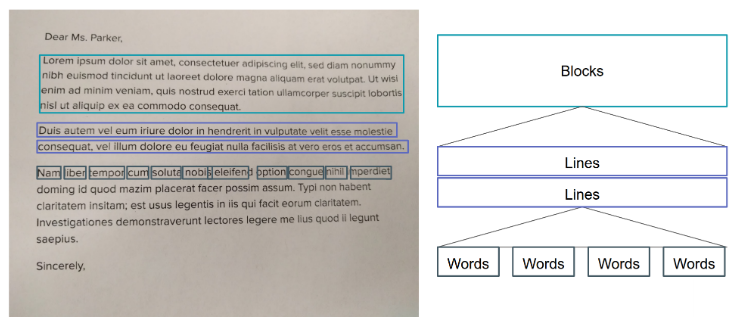
\includegraphics[width=1.0\textwidth]{Imagens/estruturatexto} 
	\caption[Reconhecimento de texto segmentado em texto em blocos, linhas e palavras.]{Reconhecimento de texto segmentado em texto em blocos, linhas e palavras.}
\fonte{\citeonline{MOBILEVISION}}	
	\label{fig:estruturatexto}
\end{figure}
